
%\documentclass[11pts,a4paper,amsmath,amssymb,floatfix]{article}%{report}%{book}
\documentclass[12pts,a4paper,amsmath,amssymb,floatfix]{article}%{report}%{book}
\usepackage{graphicx,wrapfig}% Include figure files
%\usepackage{dcolumn,enumerate}% Align table columns on decimal point
\usepackage{enumerate,enumitem}% Align table columns on decimal point
\usepackage{bm,dpfloat}% bold math
\usepackage[pdftex,bookmarks,colorlinks=true,urlcolor=rltblue,citecolor=blue]{hyperref}
\usepackage{amsfonts,amsmath,amssymb,stmaryrd,indentfirst}
\usepackage{times,psfrag}
\usepackage{natbib}
\usepackage{color}
\usepackage{units}
\usepackage{rotating}
\usepackage{multirow}

\usepackage{pifont}
\usepackage{subfigure}
\usepackage{subeqnarray}
\usepackage{ifthen} 
  
\usepackage{supertabular} 
\usepackage{moreverb}
\usepackage{fancyvrb}
\usepackage{listings}  
\usepackage{palatino} 
%\usepackage{doi}
\usepackage{longtable} 
\usepackage{float}
\usepackage{perpage}
\MakeSorted{figure}
%\usepackage{pdflscape}

\definecolor{rltblue}{rgb}{0,0,0.75}

 
%\usepackage{natbib}
\usepackage{fancyhdr} %%%%
\pagestyle{fancy}%%%%
% with this we ensure that the chapter and section
% headings are in lowercase
%%%%\renewcommand{\chaptermark}[1]{\markboth{#1}{}}
\renewcommand{\sectionmark}[1]{\markright{\thesection\ #1}}
\fancyhf{} %delete the current section for header and footer
\fancyhead[LE,RO]{\bfseries\thepage}
\fancyhead[LO]{\bfseries\rightmark}
\fancyhead[RE]{\bfseries\leftmark}
\renewcommand{\headrulewidth}{0.5pt}
% make space for the rule
\fancypagestyle{plain}{%
\fancyhead{} %get rid of the headers on plain pages
\renewcommand{\headrulewidth}{0pt} % and the line
}

\def\newblock{\hskip .11em plus .33em minus .07em}
\usepackage{color}

%\usepackage{makeidx}
%\makeindex

\setlength\textwidth      {16.cm}
\setlength\textheight     {22.6cm}
\setlength\oddsidemargin  {-0.3cm}
\setlength\evensidemargin {0.3cm}

\setlength\headheight{14.49998pt} 
\setlength\topmargin{0.0cm}
\setlength\headsep{1.cm}
\setlength\footskip{1.cm}
\setlength\parskip{0pt} 
\setlength\parindent{0pt} 

%%% 
%%% Headers and Footers
\lhead[] {\text{\small{EG3521 -- Engineering Thermodynamics}}} 
%\chead[] {\text{\small{Session 2012/13}}}  
\lfoot[]{Problem-Solving Exercise}  
%\cfoot[\thepage]{\thepage}
\rfoot[\text{\small{\thepage}}]{\thepage}
\rhead[] {{\text{\small{Session 2013/14}}}}
\renewcommand{\headrulewidth}{0.8pt}
 
%%% 
%%% space between lines
%%%
\renewcommand{\baselinestretch}{1.5}

\newenvironment{VarDescription}[1]%
  {\begin{list}{}{\renewcommand{\makelabel}[1]{\textbf{##1:}\hfil}%
    \settowidth{\labelwidth}{\textbf{#1:}}%
    \setlength{\leftmargin}{\labelwidth}\addtolength{\leftmargin}{\labelsep}}}%
  {\end{list}}

%%%%%%%%%%%%%%%%%%%%%%%%%%%%%%%%%%%%%%%%%%%
%%%%%%                              %%%%%%%
%%%%%%      NOTATION SECTION        %%%%%%%
%%%%%%                              %%%%%%%
%%%%%%%%%%%%%%%%%%%%%%%%%%%%%%%%%%%%%%%%%%%

% Text abbreviations.
\newcommand{\ie}{{\em{i.e., }}}
\newcommand{\eg}{{\em{e.g., }}}
\newcommand{\cf}{{\em{cf., }}}
\newcommand{\wrt}{with respect to}
\newcommand{\lhs}{left hand side}
\newcommand{\rhs}{right hand side}
% Commands definining mathematical notation.

% This is for quantities which are physically vectors.
\renewcommand{\vec}[1]{{\mbox{\boldmath$#1$}}}
% Physical rank 2 tensors
\newcommand{\tensor}[1]{\overline{\overline{#1}}}
% This is for vectors formed of the value of a quantity at each node.
\newcommand{\dvec}[1]{\underline{#1}}
% This is for matrices in the discrete system.
\newcommand{\mat}[1]{\mathrm{#1}}


\DeclareMathOperator{\sgn}{sgn}
\newtheorem{thm}{Theorem}[section]
\newtheorem{lemma}[thm]{Lemma}

%\newcommand\qed{\hfill\mbox{$\Box$}}
\newcommand{\re}{{\mathrm{I}\hspace{-0.2em}\mathrm{R}}}
\newcommand{\inner}[2]{\langle#1,#2\rangle}
\renewcommand\leq{\leqslant}
\renewcommand\geq{\geqslant}
\renewcommand\le{\leqslant}
\renewcommand\ge{\geqslant}
\renewcommand\epsilon{\varepsilon}
\newcommand\eps{\varepsilon}
\renewcommand\phi{\varphi}
\newcommand{\bmF}{\vec{F}}
\newcommand{\bmphi}{\vec{\phi}}
\newcommand{\bmn}{\vec{n}}
\newcommand{\bmns}{{\textrm{\scriptsize{\boldmath $n$}}}}
\newcommand{\bmi}{\vec{i}}
\newcommand{\bmj}{\vec{j}}
\newcommand{\bmk}{\vec{k}}
\newcommand{\bmx}{\vec{x}}
\newcommand{\bmu}{\vec{u}}
\newcommand{\bmv}{\vec{v}}
\newcommand{\bmr}{\vec{r}}
\newcommand{\bma}{\vec{a}}
\newcommand{\bmg}{\vec{g}}
\newcommand{\bmU}{\vec{U}}
\newcommand{\bmI}{\vec{I}}
\newcommand{\bmq}{\vec{q}}
\newcommand{\bmT}{\vec{T}}
\newcommand{\bmM}{\vec{M}}
\newcommand{\bmtau}{\vec{\tau}}
\newcommand{\bmOmega}{\vec{\Omega}}
\newcommand{\pp}{\partial}
\newcommand{\kaptens}{\tensor{\kappa}}
\newcommand{\tautens}{\tensor{\tau}}
\newcommand{\sigtens}{\tensor{\sigma}}
\newcommand{\etens}{\tensor{\dot\epsilon}}
\newcommand{\ktens}{\tensor{k}}
\newcommand{\half}{{\textstyle \frac{1}{2}}}
\newcommand{\tote}{E}
\newcommand{\inte}{e}
\newcommand{\strt}{\dot\epsilon}
\newcommand{\modu}{|\bmu|}
% Derivatives
\renewcommand{\d}{\mathrm{d}}
\newcommand{\D}{\mathrm{D}}
\newcommand{\ddx}[2][x]{\frac{\d#2}{\d#1}}
\newcommand{\ddxx}[2][x]{\frac{\d^2#2}{\d#1^2}}
\newcommand{\ddt}[2][t]{\frac{\d#2}{\d#1}}
\newcommand{\ddtt}[2][t]{\frac{\d^2#2}{\d#1^2}}
\newcommand{\ppx}[2][x]{\frac{\partial#2}{\partial#1}}
\newcommand{\ppxx}[2][x]{\frac{\partial^2#2}{\partial#1^2}}
\newcommand{\ppt}[2][t]{\frac{\partial#2}{\partial#1}}
\newcommand{\pptt}[2][t]{\frac{\partial^2#2}{\partial#1^2}}
\newcommand{\DDx}[2][x]{\frac{\D#2}{\D#1}}
\newcommand{\DDxx}[2][x]{\frac{\D^2#2}{\D#1^2}}
\newcommand{\DDt}[2][t]{\frac{\D#2}{\D#1}}
\newcommand{\DDtt}[2][t]{\frac{\D^2#2}{\D#1^2}}
% Norms
\newcommand{\Ltwo}{\ensuremath{L_2} }
% Basis functions
\newcommand{\Qone}{\ensuremath{Q_1} }
\newcommand{\Qtwo}{\ensuremath{Q_2} }
\newcommand{\Qthree}{\ensuremath{Q_3} }
\newcommand{\QN}{\ensuremath{Q_N} }
\newcommand{\Pzero}{\ensuremath{P_0} }
\newcommand{\Pone}{\ensuremath{P_1} }
\newcommand{\Ptwo}{\ensuremath{P_2} }
\newcommand{\Pthree}{\ensuremath{P_3} }
\newcommand{\PN}{\ensuremath{P_N} }
\newcommand{\Poo}{\ensuremath{P_1P_1} }
\newcommand{\PoDGPt}{\ensuremath{P_{-1}P_2} }

\newcommand{\metric}{\tensor{M}}
\newcommand{\configureflag}[1]{\texttt{#1}}

% Units
\newcommand{\m}[1][]{\unit[#1]{m}}
\newcommand{\km}[1][]{\unit[#1]{km}}
\newcommand{\s}[1][]{\unit[#1]{s}}
\newcommand{\invs}[1][]{\unit[#1]{s}\ensuremath{^{-1}}}
\newcommand{\ms}[1][]{\unit[#1]{m\ensuremath{\,}s\ensuremath{^{-1}}}}
\newcommand{\mss}[1][]{\unit[#1]{m\ensuremath{\,}s\ensuremath{^{-2}}}}
\newcommand{\K}[1][]{\unit[#1]{K}}
\newcommand{\PSU}[1][]{\unit[#1]{PSU}}
\newcommand{\Pa}[1][]{\unit[#1]{Pa}}
\newcommand{\kg}[1][]{\unit[#1]{kg}}
\newcommand{\rads}[1][]{\unit[#1]{rad\ensuremath{\,}s\ensuremath{^{-1}}}}
\newcommand{\kgmm}[1][]{\unit[#1]{kg\ensuremath{\,}m\ensuremath{^{-2}}}}
\newcommand{\kgmmm}[1][]{\unit[#1]{kg\ensuremath{\,}m\ensuremath{^{-3}}}}
\newcommand{\Nmm}[1][]{\unit[#1]{N\ensuremath{\,}m\ensuremath{^{-2}}}}

% Dimensionless numbers
\newcommand{\dimensionless}[1]{\mathrm{#1}}
\renewcommand{\Re}{\dimensionless{Re}}
\newcommand{\Ro}{\dimensionless{Ro}}
\newcommand{\Fr}{\dimensionless{Fr}}
\newcommand{\Bu}{\dimensionless{Bu}}
\newcommand{\Ri}{\dimensionless{Ri}}
\renewcommand{\Pr}{\dimensionless{Pr}}
\newcommand{\Pe}{\dimensionless{Pe}}
\newcommand{\Ek}{\dimensionless{Ek}}
\newcommand{\Gr}{\dimensionless{Gr}}
\newcommand{\Ra}{\dimensionless{Ra}}
\newcommand{\Sh}{\dimensionless{Sh}}
\newcommand{\Sc}{\dimensionless{Sc}}


% Journals
\newcommand{\IJHMT}{{\it International Journal of Heat and Mass Transfer}}
\newcommand{\NED}{{\it Nuclear Engineering and Design}}
\newcommand{\ICHMT}{{\it International Communications in Heat and Mass Transfer}}
\newcommand{\NET}{{\it Nuclear Engineering and Technology}}
\newcommand{\HT}{{\it Heat Transfer}}   
\newcommand{\IJHT}{{\it International Journal for Heat Transfer}}
%% MACROS
\newcommand{\mathbi}[1]{\boldsymbol{ #1 }}
\newcommand{\fracp}[2]{\frac{\partial #1}{\partial #2}}
\newcommand{\fracd}[2]{\frac{\mathrm{d} #1}{\mathrm{d} #2}}
\newcommand{\fracD}[2]{\frac{D #1}{D #2}}
\newcommand{\nd}[1]{\left[ #1 \right]}
\newcommand{\abs}[1]{\left| #1 \right|}
\renewcommand{\epsilon}{\varepsilon}
\newcommand{\pr}[1]{{ #1 }^\prime}
\newcommand{\br}[1]{\!\left( #1 \right)}
\newcommand{\Or}[1]{{\cal{O}}\!\left( #1 \right)}
\newcommand{\hint}{\relbar \mkern-24mu \int}
\newcommand{\nh}{{n+\frac{1}{2}}}
\newcommand{\ol}[1]{\overline{ #1 }}
\newcommand{\Uh}{\ol{U}}
\renewcommand{\d}[1]{\mathrm{d} #1}
\newcommand{\bcdot}{\ensuremath{%
  \mathchoice%
   {\mskip\thinmuskip\lower0.2ex\hbox{\scalebox{1.5}{$\cdot$}}\mskip\thinmuskip}}%
   {\mskip\thinmuskip\lower0.2ex\hbox{\scalebox{1.5}{$\cdot$}}\mskip\thinmuskip}%        
   {\lower0.3ex\hbox{\scalebox{1.2}{$\cdot$}}}%  
   {\lower0.3ex\hbox{\scalebox{1.2}{$\cdot$}}}%
}
\newcommand{\dcdot}{\mathrlap{\raisebox{1.5\depth}{$\bcdot$}}{\raisebox{-2.5\depth}{$\bcdot$}}}


\newcommand{\frc}{\displaystyle\frac}

\newlist{ExList}{enumerate}{1}
\setlist[ExList,1]{label={\bf Example 1.} {\bf \arabic*}}

\newlist{ProbList}{enumerate}{1}
\setlist[ProbList,1]{label={\bf Problem 1.} {\bf \arabic*}}

%%%%%%%%%%%%%%%%%%%%%%%%%%%%%%%%%%%%%%%%%%%
%%%%%%                              %%%%%%%
%%%%%% END OF THE NOTATION SECTION  %%%%%%%
%%%%%%                              %%%%%%%
%%%%%%%%%%%%%%%%%%%%%%%%%%%%%%%%%%%%%%%%%%%


% Cause numbering of subsubsections. 
%\setcounter{secnumdepth}{8}
%\setcounter{tocdepth}{8}

\setcounter{secnumdepth}{4}%
\setcounter{tocdepth}{4}%

\includeonly{GeneralInfo,CANum_Hicks,CA_Gomes}%,Examples_01_02,Examples_01_03}

\DeclareMathAlphabet{\mathpzc}{OT1}{pzc}{m}{it}

\begin{document}


%%%
%%%  First Page
%%%

\begin{titlepage}

\begin{center}
\bigskip
 
\vspace{4.cm}
\begin{center}
\resizebox{80mm}{!}{
\includegraphics[clip=true]{../FigBanner/UoALarge}}
\end{center}

\vspace{3.5cm}
\bigskip

{\bf {\huge  EG3521: Engineering Thermodynamics}} \\

\bigskip
{\bf {\huge Continuous Assessment}}\\
\bigskip
\vspace{1cm}
{\bf {\Large Computational Problems}}
\bigskip
\vspace{5.cm}

%{\bf {\Large Dr Jeff Gomes}}
%\bigskip

{\bf{\Large  School of Engineering}}\\
\vspace{3cm}    

\bigskip 

{\bf {\large \today}}
\end{center}
 

\end{titlepage}

\setcounter{page}{1}

\vfill

\pagebreak



\begin{center}
{\Large Computational Problem-Solving Exercise -- Individual Work}
\end{center}

\begin{enumerate}
%
\item PSE comprises solving a computational thermodynamic problem with the following deliverables: source code (Fortran, C, C++, Python or Matlab) + oral presentation. 
%
\item The PSE will be awarded either 1 or 0 CAS mark.
%
\item Source code should be submitted by email {\bf before May 2$^{nd}$ at 5pm}.  The $\lq$Subject' of the email (\href{mailto:jefferson.gomes@abdn.ac.uk}{jefferson.gomes@abdn.ac.uk}) must be $\lq$EG3521-SPE'.
%
\item (Informal) Presentation will take place during week 43.
%
\item Feedback will be given 1 week after the last presentation (before May 16).
\end{enumerate}
%





\section{Part A}

Mass conservation for a compressible gas flowing in a pipe implies
\begin{subequations}
\begin{align}
 \fracd{}{x}\left(\rho u A\right) = 0,
\end{align}
where $\rho$ is the fluid density, $u$ is the fluid velocity, $A$ is the cross sectional area of the pipe and $x$ is the distance along the pipe. In the absence of heat sources and work done by the gas, energy conservation for a compressible ideal gas flowing in a pipe implies
\begin{align}
 c_p \fracd{T}{x} + u \fracd{u}{x} - g \cos \theta,
\end{align}
where $c_p$ is the specific heat capacity of the gas at constant pressure, $T$ is the gas temperature, $g$ is the acceleration due to gravity and $\theta$ is the angle the pipe makes with the vertical. Momentum conservation implies
\begin{align}
 \rho u \fracd{u}{x} = -\fracd{p}{x} - \rho g \cos \theta,
\end{align}
where $p$ is the pressure in the pipe. This system is completed by the ideal gas equation
\begin{align}
 p = \rho R T,
\end{align}
where $R$ is the specific gas constant.
\end{subequations}

%%%%%%%%%%%%%%%%%%%%%%%%%%%
\subsubsection*{Problem 1}
Enter this system of ordinary differential equations into Matlab and solve them for suitable initial conditions when the pipe has uniform cross section. Investigate how the flow properties vary when the pipe has either a constriction or a bulge by modifying how the cross section $A\br{x}$ varies along the length of the pipe.

%%%%%%%%%%%%%%%%%%%%%%%%%%%
\subsubsection*{Problem 2}
Enter this system of ordinary differential equations into Matlab and solve them for suitable initial conditions when the pipe has uniform cross section. Investigate how the momentum equation can be modified to incorporate friction between the gas and the pipe wall, and assess how the flow properties vary when this effect is included.

\vspace{0.6cm}

\textit{Hint: in EG3007 we looked at systems of equations of the form $\fracd{\mathbi{u}}{t} = f\br{t,\,\mathbi{u}}$, where $\mathbi{u}$ is a vector of different variables. In this problem you need to solve a system of equation $M\br{\mathbi{u}} \fracd{\mathbi{u}}{t} = f\br{t,\,\mathbi{u}}$, where $M\br{\mathbi{u}}$ is a matrix. If you can form the matrix $M\br{\mathbi{u}}$, then we can reduce this system of equations to one we can solve, by premultiplying both sides by $M^{-1}$.}
%\end{document}


\section{Part B}


%%%%%%%%%%%%%%%%%%%%%%%%%%%
\subsubsection*{Problem 3}
%%%
%%% Ameen (example 3.3, pg 50)
%%%
An ice plant operates on the ideal vapour-compression cycle with superheated state using refrigerant fluid R134a.  The refrigerant enters the compressor as saturated vapour at 0.15 MPa and leaves the condenser as saturated liquid at 0.7 MPa.  Water enters the refrigerator cavity at 30$^{\text{o}}$C and leaves as ice at -5$^{\text{o}}$C. For an ice production rate of 10 kg per hour, determine the power input to the ice plant and the COP of the cycle. Also, sketch the $PH$ and $TS$ diagrams. Specific heats of ice and water are 2.1 and 4.18 kJ/(kg.K), respectively, and the latent heat of fusion of ice is 334 kJ/kg. Repeat the same procedure for ammonia and propane as refrigerat fluid. 

{\it Hint: This problem was fully solved in Tutorial 4, but here you need to generate an algorithm to solve a generic vapour-compression refrigeration cycle. Also for the thermodynamic properties, you should either (a) use external public libraries or (b) produce libraries based on spline-based lookup tables.}


 

%%%%%%%%%%%%%%%%%%%%%%%%%%%
\subsubsection*{Problem 4}
%%%
%%% Ameen (example 3.3, pg 50)
%%%
A Thermal engineer is hired to design coupled steam-power and refrigeration plants (Fig.~\ref{Ex14:Fig}). The thermal plant (I) operates 100 kg/h steam in 3-turbines reheat Rankine cycle with initial conditions and efficiencies described in Tables \ref{Ex14:Tab1} and \ref{Ex14:Tab2}. 0.1$\%$ of the power generated by the set of turbines in {\bf I} is used in the compressor of the refrigeration unit {\bf II}. The refrigeration system operates with a working fluid, $\mathcal{X}$. Tasks:
\begin{enumerate}
\item Calculate the enthalpies of all stages assuming $\mathcal{X}=\left\{\text{Ammonia and R-134a}\right\}$. 
\item For both cases, calculate the mass flow rate of the refrigerant fluid and the refrigerant capacity. 
\item Calculate the net work for the thermal cycle {\bf I} $\left(\displaystyle\frac{\dot{W}_{\text{cycle}}}{\dot{m}_{\text{water}}}\right)$ and the power produced by the set of turbines $\left(\dot{W}_{c}\right)$.
\end{enumerate}

{\it Hint: This problem is similar to Question 14 in Tutorial 4, but here you need to generate an algorithm to solve the coupled generic thermal power and vapour-compression refrigeration cycle. Also for the thermodynamic properties, you should either (a) use external public libraries or (b) produce libraries based on spline-based lookup tables.}



\begin{table}[h]
\begin{center}
\begin{tabular}{ || c || c | c ||}
\hline\hline
{\bf Flow}& {\bf Pressure}  &  {\bf Temperature}    \\
          & {\bf (bar)}     & {\bf ($^{\text{o}}$C)}       \\
\hline\hline
{\bf 1}   &   200.0         &      600                \\
{\bf 2}   &   5.0           &       --                  \\
{\bf 3}   &   5.0           &      240                 \\
{\bf 4}   &   1.0           &      --                     \\ 
{\bf 5}   &   1.0           &    99.63                    \\ 
{\bf 6}   &   0.23          &      --                     \\
{\bf 7}   &   --          &      --                     \\              
{\bf 8}   &   --           &      --                        \\
\hline \hline
{\bf 9}   &   2.0           &      --                    \\
{\bf 10}  &  16.0           &     --                     \\ 
{\bf 11}  &  --         &     --                    \\
{\bf 12}  &   --          &    --                     \\ 
\hline\hline
\end{tabular}
\end{center}
\caption{Information on the steam-power and refrigeration cycles.}\label{Ex14:Tab1}
\end{table}



\begin{table}[h]
\begin{center}
\begin{tabular}{||c | c c c c | c||}
\hline\hline
               &  {\bf Turbine 1} & {\bf Turbine 2}  & {\bf Turbine 3}  & {\bf Pump}  & {\bf Compressor}\\
{\bf Efficiency}&    0.88          &   0.85           &     0.85         &  0.92      &  1.00           \\
\hline\hline
\end{tabular}
\end{center}
\caption{Efficiencies of the equipment used in the coupled units.}\label{Ex14:Tab2}
\end{table}



\begin{figure}[h]
\begin{center}
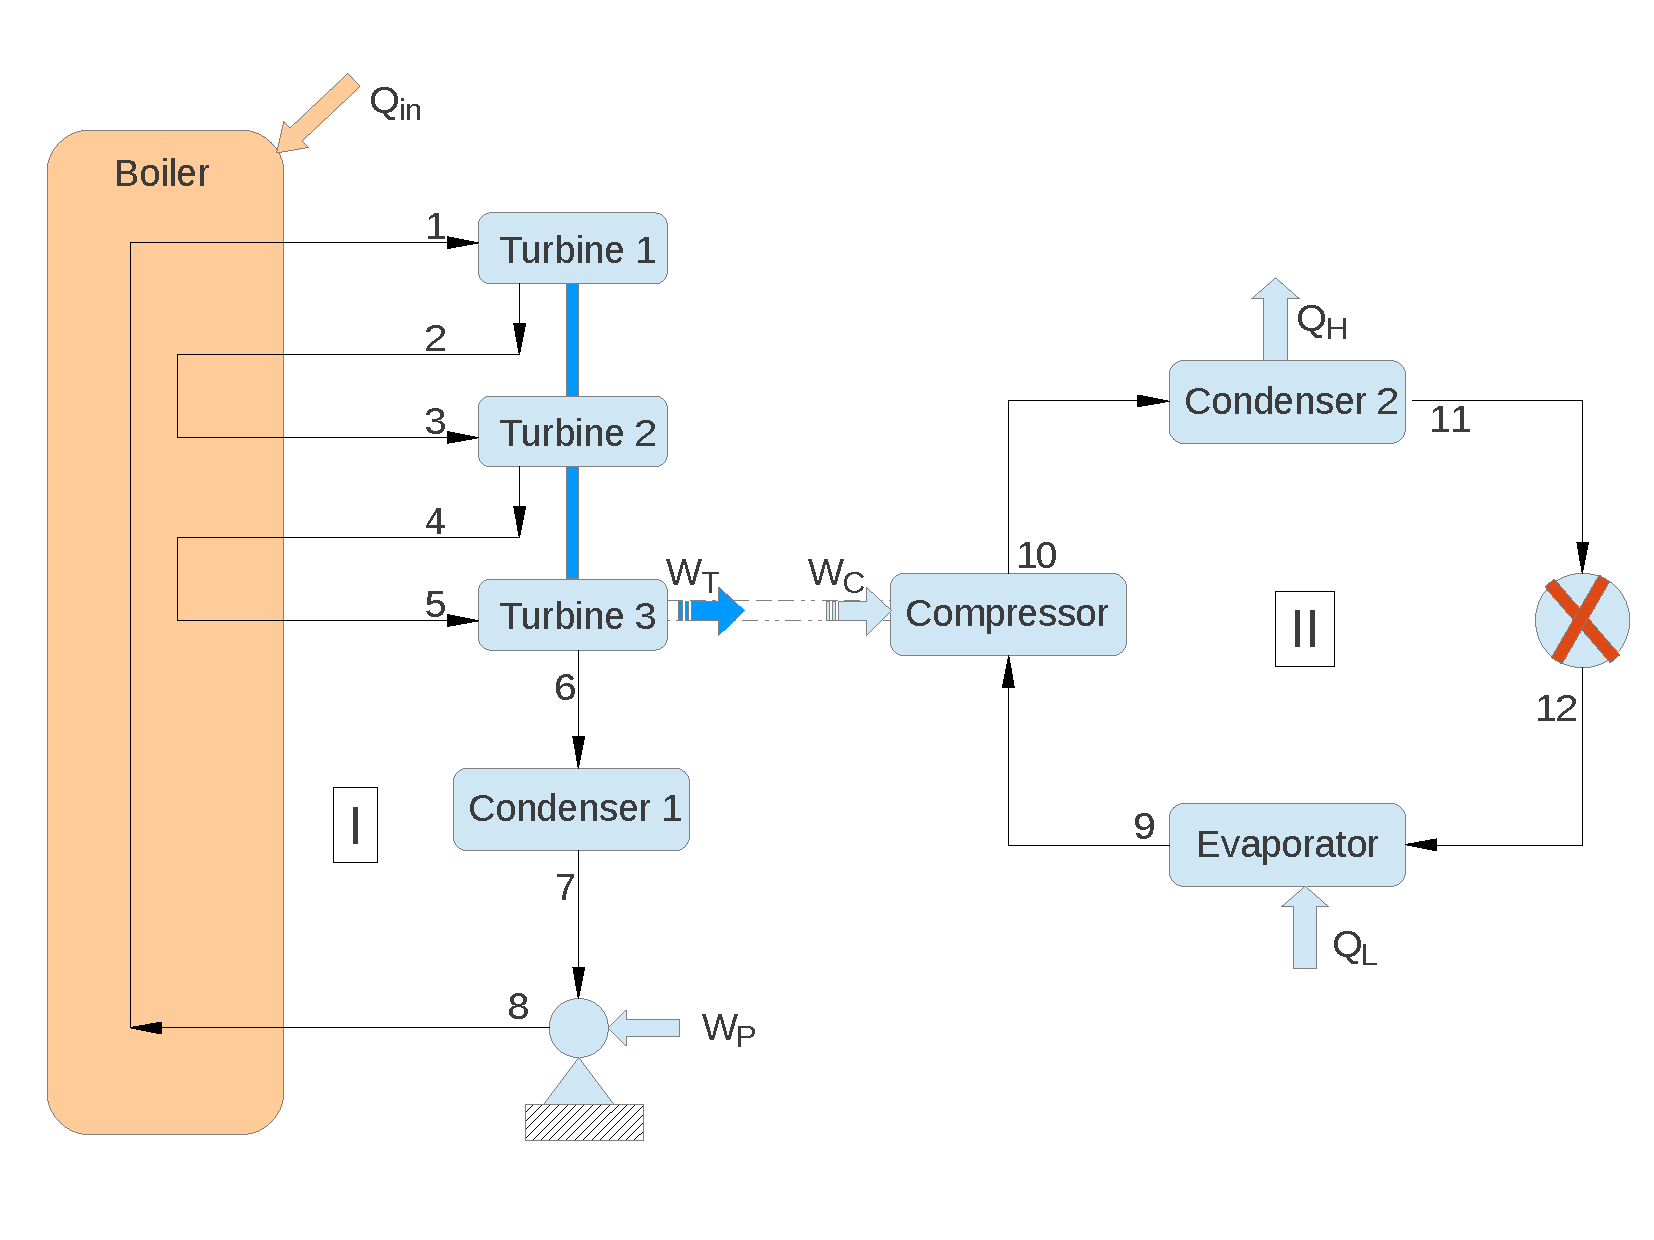
\includegraphics[width=16.0cm,height=12.0cm]{../Module_04/Pics/Overview_Refrig43}
\end{center}
\caption{Coupled reheat Rankine steam and reversed-Rankine refrigeration units.}\label{Ex14:Fig}
\end{figure}



\end{document}
